\section{ALP2}

The following changes have been made.

\subsection{ASL-676: Add \texttt{;} at the end of \texttt{if...end} statements}

Add \texttt{;} at end of block statements.
For consistency this includes: \texttt{if...end}, \texttt{while...end},
\texttt{for...end}, \texttt{try...catch...end}, \texttt{case...end},
\texttt{begin...end}.

\subsection{ASL-675: Reduce overloading of \texttt{[]}}

\subsubsection{Keep \texttt{[]} around lists of bitvector/record field
names for bit packing/unpacking}

For example:
\begin{verbatim}
var nzcv : bits(4) = PSTATE.[N,Z,C,V];
  // pack 4 x PSTATE bits into 4-bit nzcv
PSTATE.[N,Z,C,V] = nzcv;
  // unpack 4-bit nzcv into 4 x PSTATE bits
\end{verbatim}

\subsubsection{Replace \texttt{[]} around bitvectors to be concatenated
with the \texttt{::} bit-concatenation operator}

For example:
\begin{verbatim}
value = [highhalf, lowhalf]
\end{verbatim}
becomes:
\begin{verbatim}
value = highhalf :: lowhalf;
\end{verbatim}
The \texttt{::} binary operator is associative, and its precedence is
level 5 (Add-Sub-Logic).

\subsubsection{Remove support for \texttt{[]} on LHSs of assignments}

For example, the following code from \texttt{SHA256hash()}:
\begin{verbatim}
var x : bits(128);
var y : bits(128);
...
[y, x] = ROL ([y, x], 32);
\end{verbatim}
must be rewritten explicitly:
\begin{verbatim}
var x : bits(128);
var y : bits(128];
...
var tmp = ROL (y :: x, 32);
(y, x) = (tmp[1*:128], tmp[0*:128]);
\end{verbatim}

\subsubsection{Add \texttt{[:wid]} as syntactic sugar for \texttt{[0+:wid]}}

In other words, the least significant \texttt{wid} bits.

\subsubsection{Change array indexing syntax}

Change array indexing syntax from:
\begin{verbatim}
myArray[index]
\end{verbatim}
to:
\begin{verbatim}
myArray[[index]]
\end{verbatim}

\subsubsection{Use parentheses for getter/setter argument lists}

For example:
\begin{verbatim}
reg[index] = value;
\end{verbatim}
becomes:
\begin{verbatim}
reg(index) = value
\end{verbatim}

\subsection{ASL-677 and ASL-742: \texttt{integer\{-\}} syntax for inherited integer constraints}
Add a new syntax to explicitly declare integer types on the LHS of an assignment
which inherit their constraint from the RHS:

\begin{verbatim}
let Rn : bits(5) = '11111';
let i = UInt(Rn);
  // i inherits UInt() integer type and constraint {0..31}
let ui : integer = UInt(Rn);
  // ui is explicitly unconstrained integer
let ci : integer{-} = UInt(Rn);
  // NEW: ci is explicitly constrained integer,
  // inheriting constraint {0..31} from UInt()
\end{verbatim}

\subsection{ASL-624: Base values}

The current base value rules apply so long as the type of the variable or
field is unconstrained or all of the constraint's expressions use only
compile-time constants and literals.

If the variable's or field's type are parameterized or the constraint
values cannot be determined statically, then it is the programmer's
responsibility to provide an explicit initialising assignment, since a
declaration should never have an undefined value. The initialising
expression does not need to be constant, but must satisfy the
constraints.

\subsection{ASL-622: Loop/recursion limits annotations}

Inline \texttt{@looplimit} and \texttt{@recurselimit} into the loop syntax, as
optional qualifiers \texttt{looplimit} and \texttt{recurselimit}.

The presence of \texttt{looplimit} and \texttt{recurselimit} are not mandated
by the language, but a compiler should be able to optionally flag their
omission as a warning if it cannot infer the limits automatically, and some ASL
tools (such as Verilog transpilers) might treat such cases as an error.

A limit greater than or equal to $2^{128}$ is explicitly \texttt{Unbounded}.


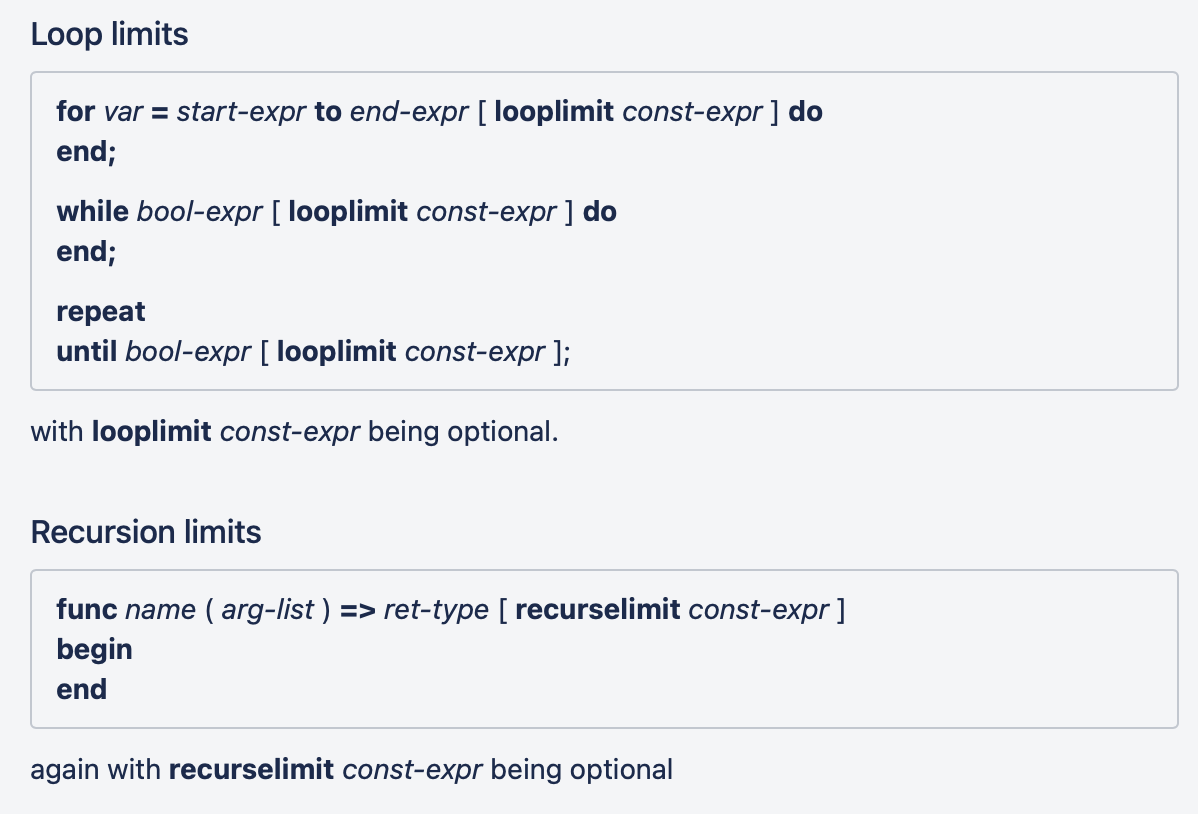
\includegraphics[width=\textwidth]{looprecurselimit.png}

\subsection{ASL-629: Define side-effects}

The order of conflicting evaluations is explicitly defined in the ASLRef
specification. A summary is as follows.

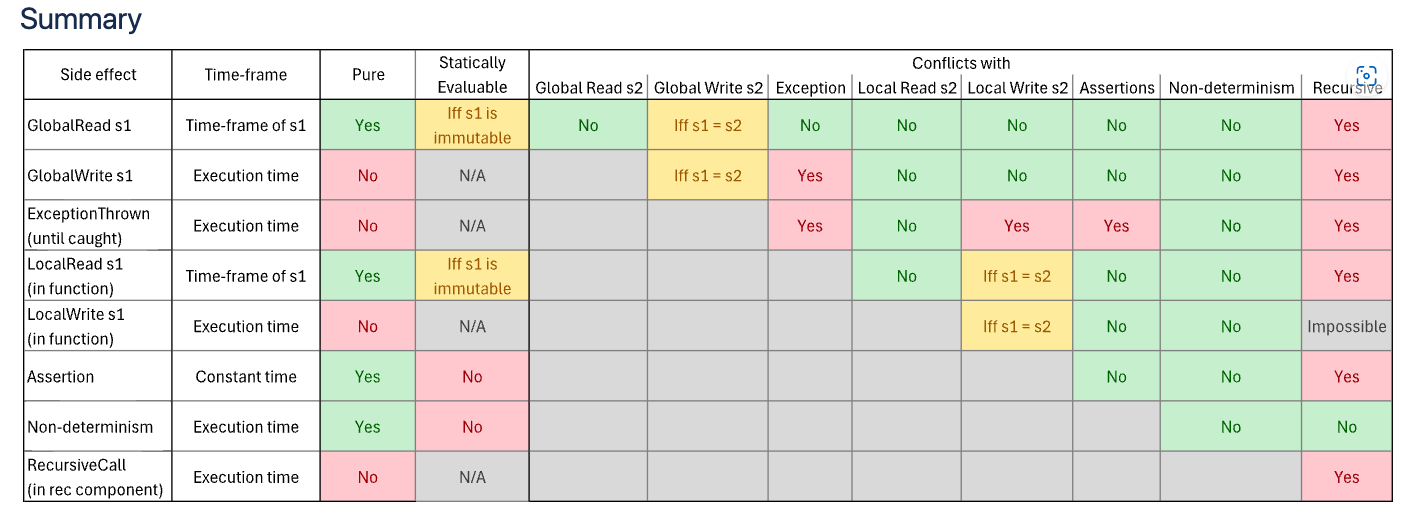
\includegraphics[width=\textwidth]{sideeffects.png}

\subsection{ASL-630: Behaviour of print}
There are two variants, \texttt{print} and \texttt{println}, which behave
as follows:
\begin{verbatim}
println("Hello world!");
println("Goodbye world!")
// Prints:
// Hello world!
// Goodbye world!
\end{verbatim}
whereas:
\begin{verbatim}
print("Hello world!");
println("Goodbye world!")
// Prints:
// Hello world!Goodbye world!
\end{verbatim}
In other words, \texttt{print} does not do any formatting such as adding any
newlines or spaces whereas \texttt{println} adds a single newline to the end of
the output.

A user can type in a series of prints to print a "concatenated" string as:
\begin{verbatim}
print("helloworld", 42); printMybitvector(mybits); println("");
\end{verbatim}

The following table summarises the supported values:\\
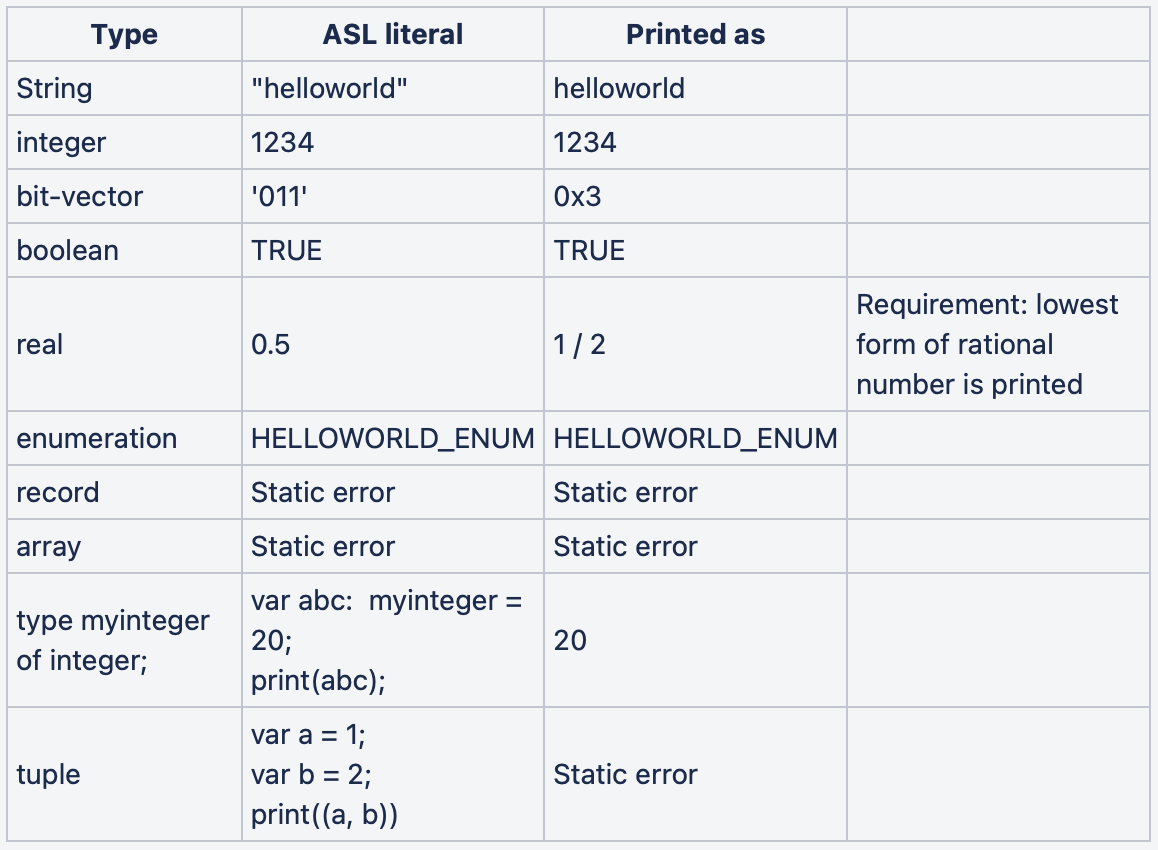
\includegraphics[width=\textwidth]{print.png}

\subsection{ASL-632: Parameters simplification}

\subsubsection{Functions must be declared with all parameters in braces}
None can be parameter-defining arguments.

\subsubsection{Parameters must be declared in a specific order}

Textually left-to-right as they appear in first the return type, then the
argument types.

\subsubsection{Functions must be called with all parameters instantiated using the braced syntax}
Except for the following (optional) cases:
\begin{itemize}
\item Standard library functions, which can omit their input parameters -
e.g. \texttt{UInt('111')}, \texttt{ZeroExtend\{64\}('111')}
\item Function calls immediately on right-hand sides of assignments where
the left-hand side is explicitly type annotated. These can inherit their
return parameter (first in the parameter list) from the left-hand side.
\end{itemize}

\subsubsection{Modify the signature of \texttt{Replicate} to align with \texttt{SignExtend} and \texttt{ZeroExtend}}

In other words, allow its parameters to be elided:
\begin{verbatim}
func Replicate{N,M}(x: bits(M)) => bits(N)
begin
  assert N MOD M == 0;
  ...
end
\end{verbatim}

\subsubsection{Call sites can elide empty argument lists \texttt{()} if
there is a non-empty parameter list}
For example, \texttt{Zeros\{64\}}. However, this cannot
be applied in conjunction with an elided single parameter on RHS.

\noindent
Examples:
\begin{verbatim}
// func Bar{N}(...) => bits(N)
// func Baz{A,B}(...) => bits(A)
let res : bits(N) = Bar{}(args);
  // omitted single parameter N (no ambiguity)
  // desugared to Bar{N}(args);
let res : bits(N) = Baz{,sz}(bv);
  // omitted positional parameter A
  // desugared to Baz{N,sz}(bv);
let res : bits(N) = Baz{}(bv);
  // ILLEGAL - only first parameter can be omitted

func{_}(..., x : bits(M), ..., y : bits(N)) => bits(L)
  // Parameters must be declared {L,M,N}

let res = Zeros{64};
  // can avoid empty argument list ()
let res : bits(64) = Zeros{}();
  // OK
let res : bits(64) = Zeros{64};
  // OK
let res : bits(64) = Zeros{};
  // INVALID - parsing conflict with empty record

let - = UInt('1111');
  // equivalent to UInt{4}('1111');
// func ZeroExtend{N,M}(x: bits(M)) => bits(N)
// no need to specify input parameter M
let - : bits(64) = ZeroExtend{64}('11');
  // equivalent to ZeroExtend{64,2}
let - : bits(64) = ZeroExtend{}('11');
  // can also elide the output parameter N
\end{verbatim}

\subsection{ASL-710: Syntax for \texttt{IN '10xx'}}

\subsubsection{Require that the \texttt{IN} set membership operator always
requires \{ and \} around the set}

This is regardless of the number of members.

In other words, forbid removal of \texttt{\{} and \texttt{\}} around a
single-member set---the following used to be permitted by ASL1 for
single-member sets but is not anymore:

\begin{itemize}
\item \texttt{Mybits IN \{'000x'\}} could be written as \texttt{Mybits IN '000x'}
\item \texttt{!Mybits IN \{'000x'\}} could be written as \texttt{!Mybits
IN '000x'}
\end{itemize}

\subsubsection{Reintroduce ASL0 syntactic sugar}

This means that:
\begin{itemize}
\item \texttt{Mybits IN \{'000x'\}} can be written as \texttt{Mybits == '000x'}
\item \texttt{!Mybits IN \{'000x'\}} can be written as \texttt{Mybits != '000x'}
\end{itemize}

\subsection{ASL-738: Rename \texttt{UNKNOWN} to \texttt{ARBITRARY}}

\texttt{UNKNOWN} keyword is renamed to \texttt{ARBITRARY}.


\subsection{ASL-637: Dynamic and static errors}

The taxonomy of ASL errors as dynamic or static has been captured in the ASLRef
specification. A summary is as follows.

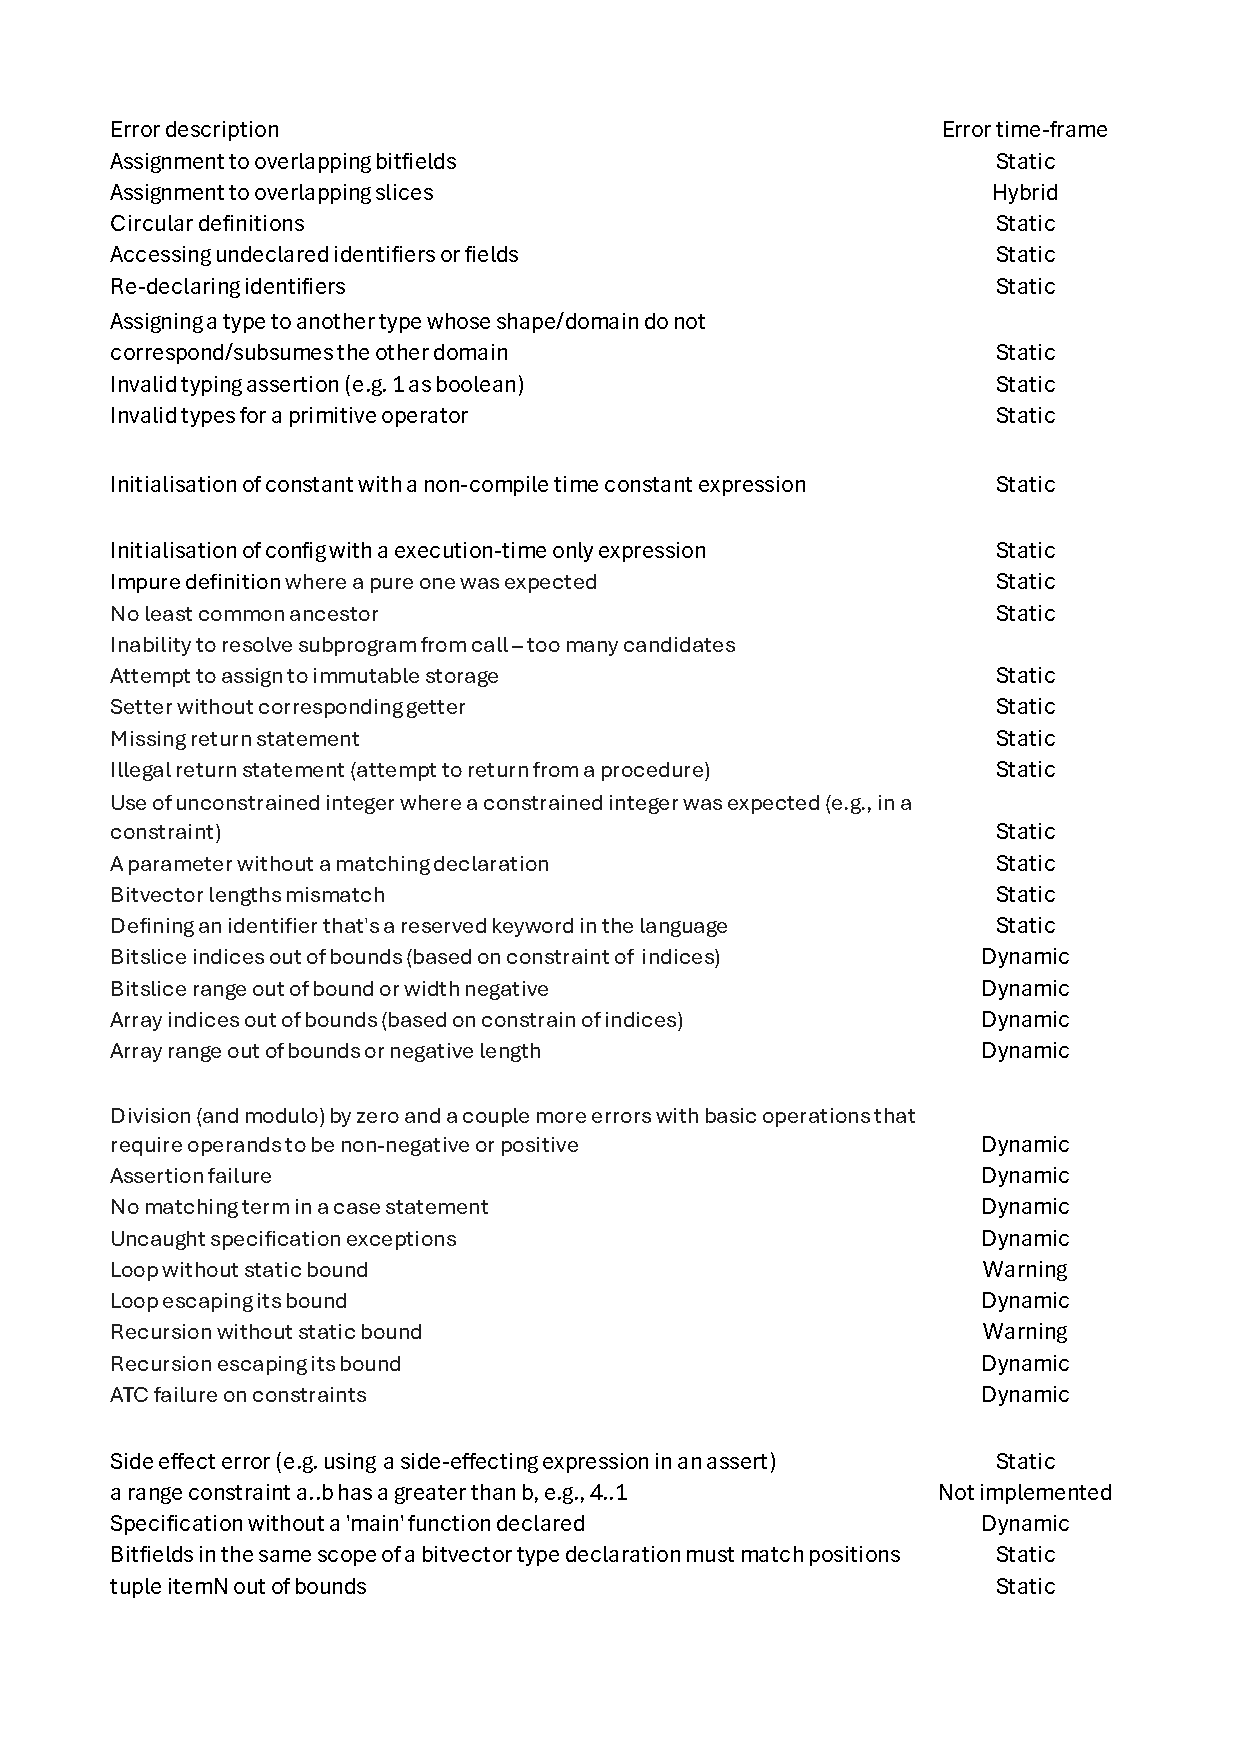
\includegraphics[width=\textwidth]{ASL-error-status.pdf}

\subsection{ASL-702: Underscore identifiers}

Any identifier with a double-underscore (\texttt{\_\_}) prefix is
treated as a static error by ASLRef. Other compilers might recognise
these identifiers as keywords for compiler-specific extensions.

Any identifier with a single underscore followed by an alphanumeric
character is treated as a normal identifier, but ASLRef recommends that
these are only for use by platform-specific code which should not clash
with the rest of a portable ASL program.

The following keywords are removed from the ASL reserved list:
\begin{verbatim}
access
advice
after
aspect
before
entry
expression
get
is
pattern
pointcut
replace
set
statements
watch
\end{verbatim}

\subsection{ASL-741: Behaviour of \texttt{ARBITRARY}}

Clarify behaviour of \texttt{ARBITRARY} as follows:

Each evaluation can produce a different arbitrary value, but (as always)
once a particular expression is evaluated, its arbitrary value cannot
change. This is because evaluation produces native values, and
\texttt{ARBITRARY} is not a valid native value - so once evaluated, it
becomes an unchanging native value like any other.  Note that there are
two important consequences of producing an arbitrary value when
evaluating expressions of the form \texttt{ARBITRARY : type}:
\begin{enumerate}
\item The arbitrary value depends only on type, and no other ASL storage
elements.

\item The only guarantee of the resulting value is that it is a valid member of
type. In particular, the language does not define which valid member it
is, and ASL specifications must not rely on the value (for example, there
is no way to test whether a value was produced by evaluating
\texttt{ARBITRARY}).
\end{enumerate}

\subsection{ASL-706: Getters and setters simplification}

\subsubsection{Forbid getters and setters without an argument list}

Although that list could be empty.

\subsubsection{Restrict setter usage on some left-hand sides}

For example, no setters in tuples.

\subsection{ASL-744: Clarifying left-hand sides}

\subsubsection{Mutable assignments}

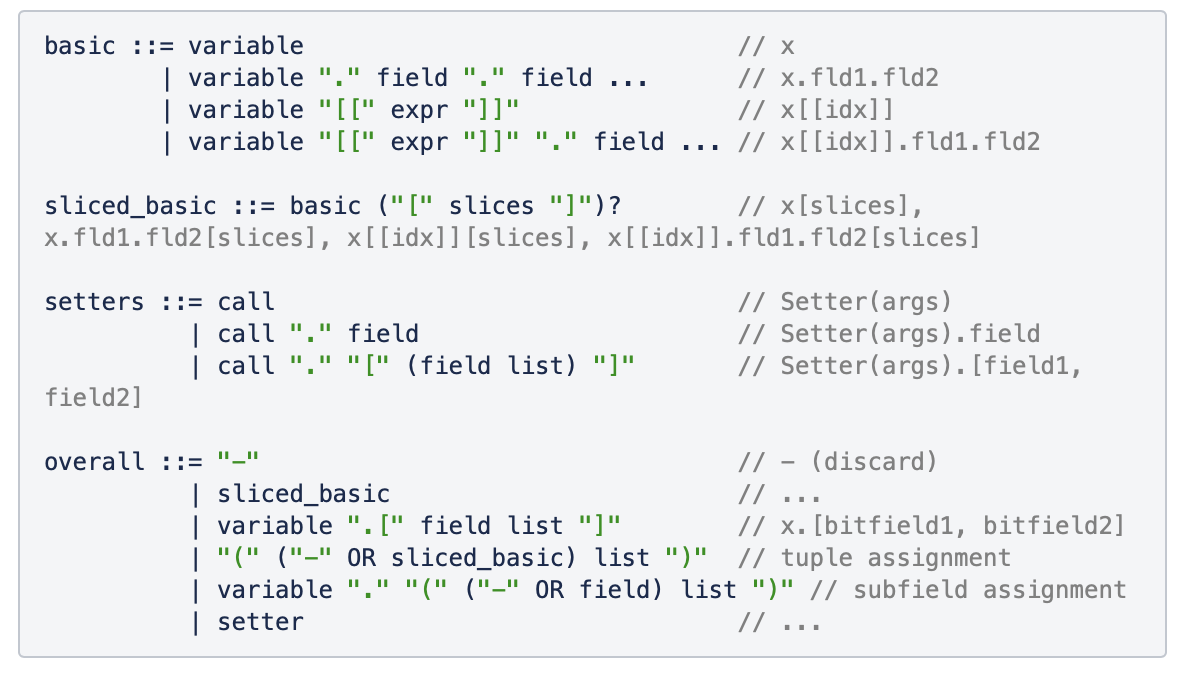
\includegraphics[width=\textwidth]{lhs-multiple.png}

\subsubsection{Declarations}

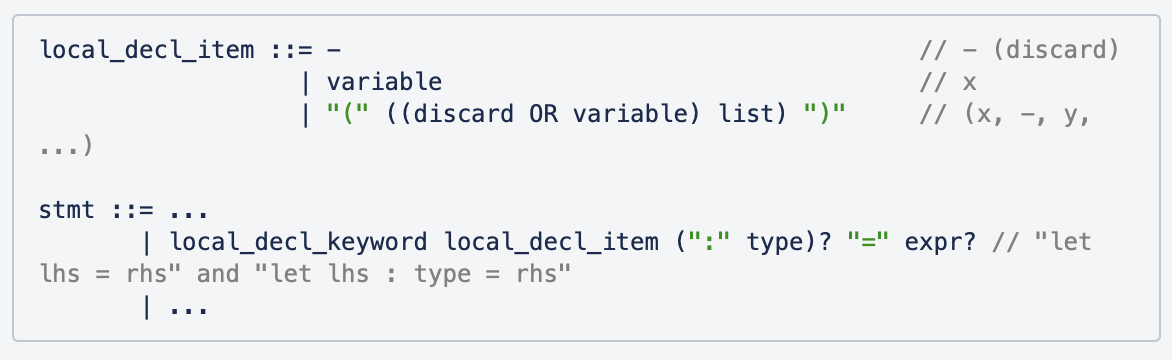
\includegraphics[width=\textwidth]{lhs-declarations.png}

\subsection{ASL-596: Remove \texttt{Int()} and \texttt{IsZeroBit()} in the standard library}

\subsection{ASL-539: Nested bitfields}

\subsubsection{Ensure that nested bitfields checks in ASLRef handle the following patterns}

\begin{verbatim}
type Nested_Type of bits(32) {
    [31:16] fmt0 {
        [15] : fixed,
        [14] : moving
    },
    [31:16] fmt1 {
        [15] : fixed,
        [0]  : moving
    },
    [31] : fixed,
    [0]  : fmt
};

var nested : Nested_Type;

// select the correct view of moving
// nested.fmt is '0'
//    nested.fmt0.moving is nested[30]
// nested.fmt is '1'
//    nested.fmt1.moving is nested[16]
let moving = if nested.fmt == '0' then
               nested.fmt0.moving
             else
               nested.fmt1.moving;

// below are all equivalent
let fixed = nested[31];
let fixed = nested.fixed;
let fixed = nested.fmt0.fixed;
let fixed = nested.fmt1.fixed;
\end{verbatim}

\subsubsection{Require that fields with same name occupy the same absolute bit
positions in all ancestor fields}

This will result in a static error if this requirement is not met.
